\documentclass[12pt]{article}

\usepackage{authblk} % Title, Author, and Affiliation formatting
\usepackage[utf8]{inputenc}
\usepackage{datetime} % Time and Date Formatting
\usepackage{graphicx}
\usepackage{tfrupee}
\usepackage{amsmath}
\usepackage{amssymb}
\usepackage{hyperref}
\graphicspath{ {/home/ryan/Desktop/math_assessment} }

\topmargin = 0cm
\evensidemargin = -1cm
\oddsidemargin = -1cm
\textheight = 23cm
\textwidth = 18cm

\title{\vspace{-3.5cm}\Huge{\underline{\textbf{Internal Assessment Task}} \\ Data Interpretation \& Reasoning}}
\author{\vspace{-3mm}Ryan Chowdhary}
\affil{\vspace{-4mm}{\small{\it X `D', Roll no. 17, SOSE DWARKA SEC-10 }}}
\date{\vspace{-0.75cm}\today}

\begin{document}

\maketitle

\section{Introduction}
Statistics can also be termed as data handling. It is a process of drawing facts from numerical data. It includes collection, presentation and interpretation of the data. Gathering information in the form of number or numerical figures is called data.
In this project we will make use of data handling on real life datasets.

\section{Objectives}
Exploring the Practical Applications of Statistics and Probability in Real-Life Situations and Demonstrating the Importance of Accurate Data Interpretation.

\section{Acknowledgement}
I would like to express my special thanks of gratitude to my Mathematics teacher "Mr. Pradeep Jindal" for their able fuidance and support in completing my project.
I would also like to extend my gratude to the Principal Sir ``Dr. Atul Kumar'' and Vice Principal Ma'am ``Dr. Ranjita'' for providing me with all the facility that was required.

Date: \today

\pagebreak

\section{Important Definitions}

\subsection{Mean}
In statistics, the mean is one of the measures of central tendency, apart from the mode and median. Mean is nothing but the average of the given set of values. It denotes the equal distribution of values for a given data set.\\
it is denoted by $\bar{x}$\\
the general formula for calculating mean is:
$$ \bar{x} = \frac{1}{n}\sum_{i=1}^nx_i $$
where, n = number of observations, $x_i$ = value of element $i$\\
other formulas include\\
\textbf{Assumed Mean Method (Short-Cut Method):}
$$ \bar{x} = A + \frac{1}{n}\sum^n_{i=1}f_id_i $$
\begin{itemize}
    \item A = Assumed Mean
    \item $d_i$ = deviation
    \item $f_i$ = frequency of $d_i$
\end{itemize}
it is best used when value of $f_ix_i$ is nither too big or too small\\
\textbf{Step-Deviation Mean Method:}
$$ \bar{x} = A + h\left\{\frac{1}{n}\sum_{i=1}^nf_iu_i\right\} $$
\begin{itemize}
    \item $h$ = class interval size
    \item $u_i$ = unit interval
    \item $f_i$ = frequency of $u_i$
\end{itemize}
it is best used when the value of $f_ix_i$ is too big for us to apply any of the formulas mentioned above\\

\subsection{Median}
Median, in statistics, is the middle value of the given list of data when arranged in an order. The arrangement of data or observations can be made either in ascending order or descending order.\\
the general method for finding the median is
taking n is number of observations
\begin{itemize}
    \item \textbf{if n is odd: }
    then median is the value of $\left(\frac{n+1}{2}\right)^{th}$ observation
    \item \textbf{if n is even: }
    then median is the AM of the values of $\left(\frac{n}{2}\right)^{th}$ and $\left(\frac{n}{2} + 1\right)^{th}$ observations.
\end{itemize}

\subsection{Mode}
In statistics, the mode is the value that is repeatedly occurring in a given set. We can also say that the value or number in a data set, which has a high frequency or appears more frequently, is called mode or modal value. \\
It is one of the three measures of central tendency, apart from mean and median. For example, the mode of the set ${3, 7, 8, 8, 9}$, is $8$. \\
Therefore, for a finite number of observations, we can easily find the mode. A set of values may have one mode or more than one mode or no mode at all.\\
\begin{itemize}
    \item  \textbf{for grouped data:}
    $$ Mode = l + \left(\frac{f_1 - f_0}{2f_-f_0-f_2}\right)\times h $$
    \begin{itemize}
        \item $l$ = lower limit of the modal class
        \item $h$ = size of the class interval
        \item $f_1$ = frequency of the modal class
        \item $f_0$ = frequency of the class preceding the modal class
        \item $f_2$ = frequency of the class succeeding the modal class
    \end{itemize}
    \item \textbf{for un-grouped data:}
    The value occurring most frequently in a set of observations is its mode. In other words, the mode of data is the observation having the highest frequency in a set of data. There is a possibility that more than one observation has the same frequency, i.e. a data set could have more than one mode. In such a case, the set of data is said to be multimodal.
\end{itemize}
\subsection{Probability}
Probabilitymeans possibility. It is a branch of mathematics that deals with the occurrence of a random event. \\
The value is expressed from zero to one. Probability has been introduced in Maths to predict how likely events are to happen.\\
The meaning of probability is basicallythe extent to which something is likely to happen.\\
This is the basic probability theory.\\
\begin{itemize}
    \item \textbf{Formula:}
    $$ Probability \; of \; event \;to \;happen \;P(E) = \frac{Number \;of \;favourable \;outcomes}{Total \;Number \;of \;outcomes}$$
    $$ P(E) = \frac{n(E)}{n(S)} $$
\end{itemize}
\pagebreak

\section{\Huge{Challenges}}
\subsection{Set 1: House Prices Across Delhi}
The first Dataset chosen is a collection of house prices across Delhi.
\\
\begin{figure}[h]
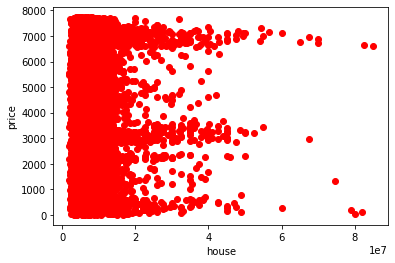
\includegraphics[width=11cm]{housing_prices_in_delhi.png}
\centering
\caption{This figure represents the housing prices across Delhi.}
\end{figure}
\\
\paragraph{Mean: }
First we shall find the mean housing price. \\
because the values are very large, we will use Step-deviation Mean method \\
\begin{equation}
\bar{x} = A + h \left\{ \frac{1}{n} \sum_{i=1}^nf_iu_i\right\}, \; u_i = \frac{x_i - A}{h}
 \end{equation}
here, $h$ is the class interval, $x_i$ is the value of element $i$ and $A$ is the assumed mean, $n$ is the total number of observations, and $u_i$ is the unit interval \\
for this calculation we will take $a = 2600000$, and $h = 1$ as it is a ungrouped data.
\begin{equation}
\begin{aligned}
\bar{x} = A + \left[\frac{\sum u_i}{n}\right] \\ \implies \bar{x} = 2600000 + \frac{34980670000}{7738} \\ \implies \bar{x} = 8320634.53
\end{aligned}
\end{equation}
$\therefore$ the mean price for a house in Delhi is \rupee $83,20,634.53$

\paragraph{Median: }
since the number of observations is even, the median house price is the mean of $\left(\frac{n}{2}\right)^{th}$ and $\left(\frac{n}{2} + 1 \right)^{th}$ observation.
$$\therefore median = \frac{\left(9900000 + 2600000\right)}{2} = 6250000$$
the median price is \rupee $62,50,000$ \\
\paragraph{Mode: }
And because the mode is the observation with the highest frequency, there will be no modal value for the given data set as no value is repeating more than once.

\pagebreak

\subsection{Set 2: Infant Mortality Rate Around The World in 2019}

\begin{figure}[h]
\centering
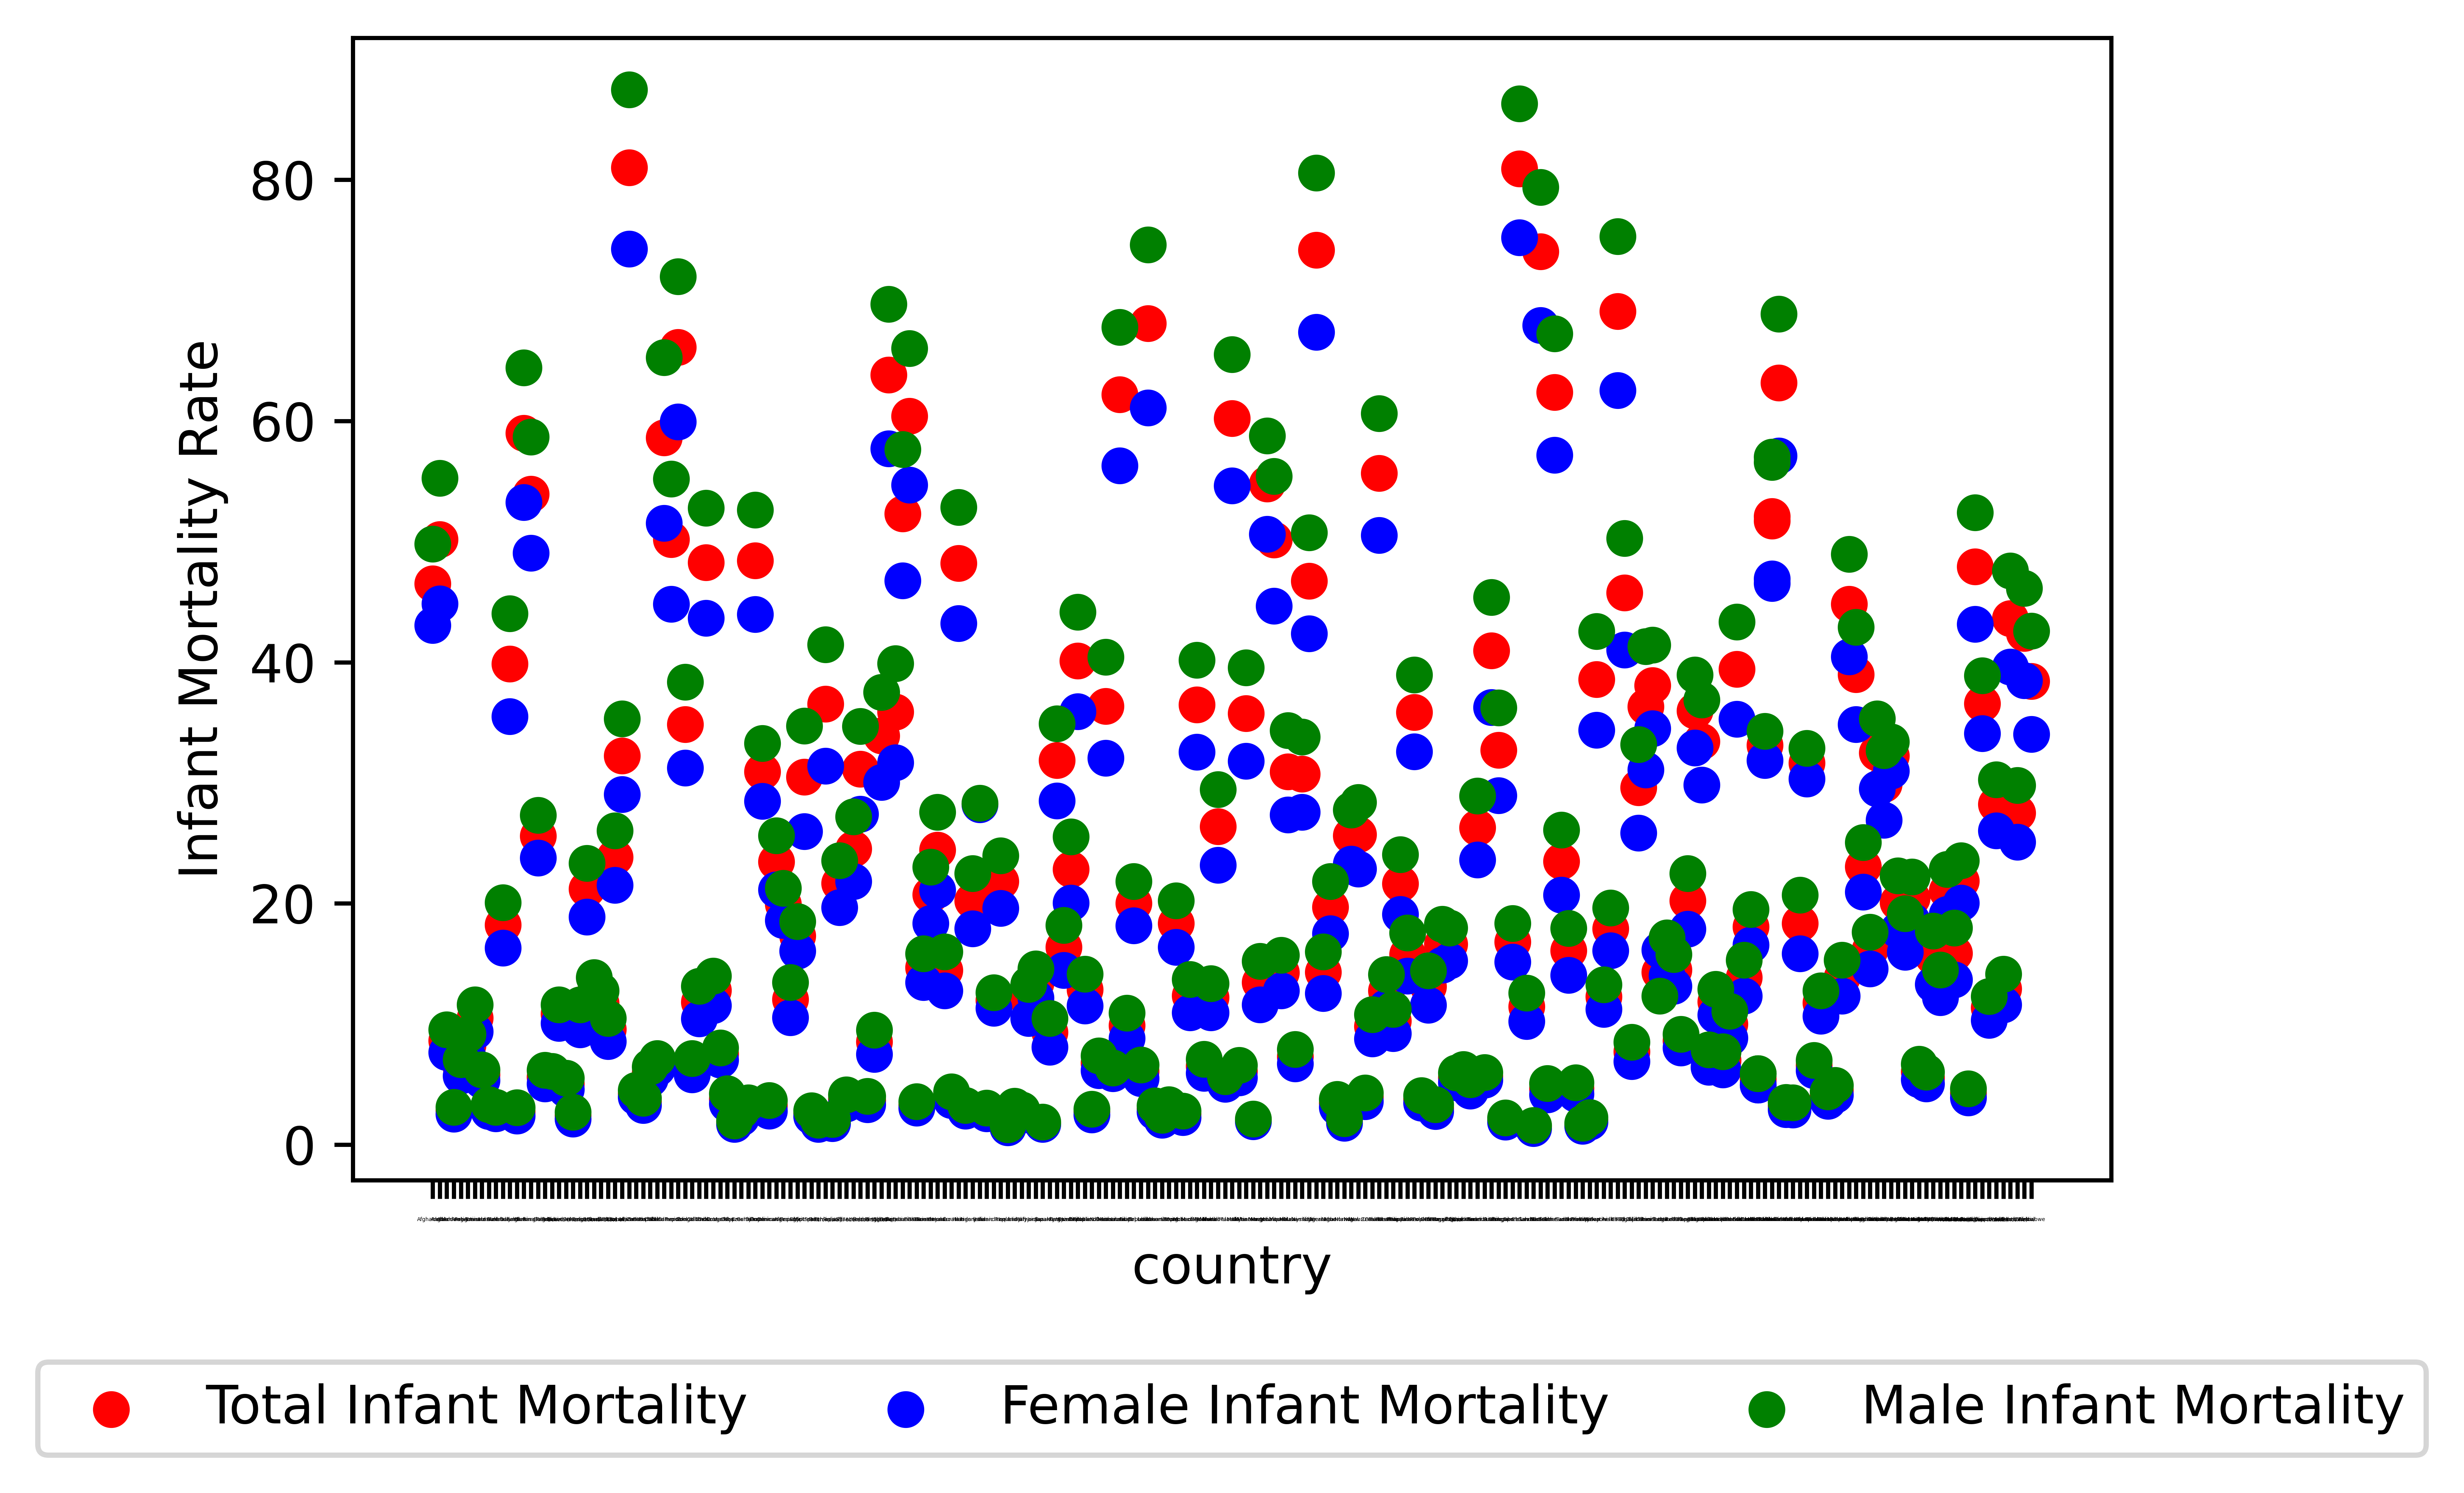
\includegraphics[width=15cm]{Infant Mortality Rate}
\caption{Shows the Infant Mortality Rate of Boys and Girls in 2019 against the Country they are obtained from.}
\end{figure}

\paragraph{Mean: }
Same as in the previous data set, this one is a ungrouped dataset as well.\\
because, the values of $x_i$ are nither too big or too small, we will use the assumed mean method also called Short-Cut Method.

$$ \bar{x} = A + \frac{1}{N} \sum_{i=1}^{n}f_id_i$$
where, $d_i$ is the deviation of $x_i$ and $n$ is the total number of observations\\
because, the given dataset is ungrouped, $f_i$ for all $x_i$ will be $1$\\
Mean Mortality Rate among Countries:\\
Taking $A = 30$\\
$d_i = x_i - A$
\begin{equation}
\begin{aligned}
\bar{x} =  A + \frac{1}{N} \sum_{i=1}^n d_i \\ \implies \bar{x} = 30 + \frac{-2041.9}{231} \\ \implies \bar{x} = 21.16
\end{aligned}
\end{equation}
$\therefore$ the mean Infant Mortality rate in the world is $21.16$\%\\
Similarly, for boys:
$A = 27.5$
\begin{equation}
\bar{x} =  27.5 + \frac{-1012.58}{231} = 23.11\%
\end{equation}

And Girls:
$A = 34.7$
\begin{equation}
\bar{x} = 34.7 + \frac{-3604.55}{231} = 19.09\%
\end{equation}
meaning that, 23 boys and 19 girls out of every 100 boys and girls respectively have died in 2019.\\

\paragraph{Median: }
because, the number of observations is odd, the middle term i.e. $\left(\frac{n+1}{2}\right)^{th}$ observation is the median.\\
$$\therefore median \; Infant \; Mortality \; rate = \left(\frac{231 + 1}{2}\right)^{th} observation = 14.48$$
same for boys and girls\\
$$ median \; mortality \; rate \; boys = \frac{231 + 1}{2}^{th} observation = 15.98\% $$

$$ median \; mortality \; rate \; girls = \frac{231 + 1}{2}^{th} observation = 13.29\% $$
\paragraph{Mode: }
the mode is the observation with the highest frequency \\
$\therefore$ the mode or modal Infant Mortality rate is 13.89\%\\

\paragraph{Probability: }
From the above calculation, the probability of a child dying is 21.16\% in 2019,
$$ P(child \; dying) = \frac{21.16}{100} $$
$\therefore$ 21 out of 100 cases the death of the Infant.\\


\pagebreak

\section{Refrences}
\begin{itemize}
    \item NCERT Class 10 Mathematics
    \item R.D. Sharma Class 10 Mathematics
    \item Python, Pandas for data preparation and visualization
    \item $1^{st}$ dataset \url{www.kaggle.com/datasets/goelyash/housing-price-dataset-of-delhiindia}
    \item $2^{nd}$ dataset \url{www.kaggle.com/datasets/komalkhetlani/infant-mortality}
\end{itemize}

\end{document}